
%(BEGIN_QUESTION)
% Copyright 2011, Tony R. Kuphaldt, released under the Creative Commons Attribution License (v 1.0)
% This means you may do almost anything with this work of mine, so long as you give me proper credit

This solar hot-air collector bank uses a variable-speed fan as the final control element, the temperature controller commanding the fan to blow air at different rates in order to maintain a relatively constant discharge temperature.  The hot air is being used to dehydrate wheat grain prior to grinding it into wheat flour.  Unfortunately, this system is not operating as it should -- the grain is taking longer to dry out than it usually does, despite enjoying the same amount of sunlight (heat source) as it has in the past:

$$\includegraphics[width=15.5cm]{i01699x01.eps}$$

A fellow instrument technician proposes that the VFD is causing the blower motor to spin at the wrong speed, while an operator thinks the solar collectors' glass panes probably need to be cleaned of dust and dirt accumulation.  Explain why both of these hypotheses are incorrect, and suggest at least two of your own hypotheses to account for the what we see happening in this system.

\vskip 20pt \vbox{\hrule \hbox{\strut \vrule{} {\bf Suggestions for Socratic discussion} \vrule} \hrule}

\begin{itemize}
\item{} A valuable principle to apply in a diagnostic scenario such as this is {\it correspondence}: identifying which field variables correspond with their respective controller faceplate displays, and which do not.
\item{} Determine the proper action for this loop controller (direct or reverse).
\item{} Why is the temperature gain less for each successive panel?  Is this a problem, or do you think this is how the system normally operates?
\end{itemize}

\underbar{file i01699}
%(END_QUESTION)





%(BEGIN_ANSWER)


%(END_ANSWER)





%(BEGIN_NOTES)

The TIC's PV display reads higher than the TI on the discharge of the collector array.  Since we know the grain is taking too long to dry, the lower indication (TI) is more believable than the TIC.  This suggests a problem with either the TE, TT, or TIC input causing the TIC to register a falsely-high temperature.

%INDEX% Process: solar hot-air collector control system

%(END_NOTES)


